\section{Bilder} \label{sec:bilder}
Bilder i programmet følger med boligobjektet, bildene blir heller \underline{ikke} lagret i selve objektet og serialiseres derfor \underline{ikke}. Referanse til bildemappen er lik static variabeln \texttt{objektID}. Første bilde som brukeren laster opp blir brukt på fremsiden ved presentasjon av boligen. Fremsidebilde blir plassert i boligmappen som 1.jpg. Men dersom brukeren velger å laste opp flere bilder får de inkrementelle navn som 2.jpg, 3.jpg og så videre. 

\subsection{Bildeklasser}
\subsubsection*{Bildefilsti.java}
Primær oppgave for klassen er å sørge for at programmer får en absolutt filsti til hvor alle bilder er lagret uavhengig operativsystem. Metodene i de klasse returnerer en \texttt{String} som benyttes i \texttt{File()} objekter i flere klasser i programmet.  
Klassen ble opprettet på grunn av at html visninger stiler krav på en absolutist filsti for \texttt{html} som begynner med en "<file:"> prefiks. 
Derfor metoder i klassen kan: 
\begin{itemize}[noitemsep,nolistsep]
\item Returnere plassering til \texttt{programdata/img/} uavhengig operativsystem.
\item Returnere filsti til et standard bilde som vises dersom brukeren ikke laster opp egne bilder.
\item Gitt et boligobjekt:
\begin{itemize}
\item Filsti til boligens fremsidebilde som kan brukes i File() og som html sti\footnote{Som beskrevet over blir strengen returnert med prefix "<file:">}
\item Filsti til boligens gallerimappe og som html sti
\end{itemize}
\end{itemize}

\subsubsection*{BoligBilde.java}
Klassen brukes til bildebahendlig og opplastning av bilder til eksisterende boligobjekter. Metoder i klassen (1) kontrollerer antall allerede opplastede bilder for boligen, (2) leser inn nytt bilde fra harddisk (gitt et \texttt{File()} objekt), (3) endrer størrelsen på bildet slik at det blir tilpasset den visning som brukes i programmet (samt for å holde størrelsen nede på bildemappen), (4) lagrer behandlet bile i gallerimappen for boligen.

\subsection{Lagring av bilder}
Lagring av bilder er ikke serialisert hvilket medfører at alle bilder blir lagret som bildefiler i \texttt{programdata/img/boligbilder/\textbf{objektID}}. For hvert nytt boligobjekt som blir oprettet lages det en ny mappe med samme navn som \texttt{objektID} i \texttt{programdata/img/boligbilder/}. Dette gjør at serialisering av bildeobjekter er ikke nødvendig, deretter start og avslutting av programmet blir betydelig raskere\footnote{Avhengig av hvor mange bolig objekter som er lagret i registrene.}. Etter at bildemappe er opprettet kan brukeren legge til bilder for boligen. Det blir foretatt følgende trinn ved opplasting av et bilde for en bolig:
\begin{enumerate}[noitemsep,nolistsep]

\item Fra vindu for boligregistrering/endring brukeren initierer \texttt{JFileChooser}, dersom man velger å laste opp bilder. Her blir det gjort forskjell på hvis dette er en ny, eller en eksisterende bolig. Hvis det er en ny bolig blir brukeren presentert med en dialog som spør om opplasting av bilder etter at registreringen blitt foretatt.

\item Dersom brukeren laster opp en ny fil blir den buffret som \texttt{BufferedImage} og skalert til mindre dimensjoner, eksepel \ref{kode:innlesningbilde} og \ref{kode:bildestorrelse}.

\item Etter endring av størrelse blir bildet lagret med et inkrementelt filnummer (forrige bilde som ble lastet opp + 1). Dersom det ikke finnes tidligere bilder blir det første opplastede bilde satt til 1.jpg, eksempel \ref{kode:bildelagring}.

\end{enumerate}

\begin{lstlisting}[caption=BoligBilde.java: Innlesning av bildefil, label=kode:innlesningbilde]
	private void lesInnBilde(File bildeFil) throws IOException {
        bilde = ImageIO.read(bildeFil);
        bildeType = bilde.getType() == 0 ? BufferedImage.TYPE_INT_ARGB : bilde.getType();
    }
\end{lstlisting}

\begin{lstlisting}[caption=BoligBilde.java: Endring av opplastet bildestørrelse, label=kode:bildestorrelse]
	private BufferedImage endreBildeTilStandardStorrelse(BufferedImage originalBilde, int bildeType) {
        BufferedImage nyttBilde = new BufferedImage(Konstanter.BILDE_WIDTH, Konstanter.BILDE_HEIGHT, bildeType);
        Graphics2D grafikk = nyttBilde.createGraphics();
        grafikk.drawImage(originalBilde, 0, 0, Konstanter.BILDE_WIDTH, Konstanter.BILDE_HEIGHT, null);
        grafikk.dispose();
        return nyttBilde;
    }
\end{lstlisting}

\begin{lstlisting}[caption=BoligBilde.java: Lagring av et nytt eller tillegsbilde for en bolig, label=kode:bildelagring]
	private void lagreBilde(BufferedImage bilde, String path) throws IOException {
        ImageIO.write(bilde, "jpg", new File(path));
    }

	public void lagreNyttBildeForBolig(Bolig bolig, File innlestFil) throws IOException {
        lesInnBilde(innlestFil);
        BufferedImage tmpBilde = endreBildeTilStandardStorrelse(bilde, bildeType);
        String galleriSti = getGalleriSti(bolig);
        String fullSti = galleriSti + "/" + String.valueOf(getNesteFilnummer(bolig)) + ".jpg";
        lagreBilde(tmpBilde, fullSti);
    }
\end{lstlisting}

\subsection{Visning av bilder}
Bildevisning kan initialiseres på to måter: 
\begin{enumerate}
\item Fra vindu for boligbehandling, figur \ref{fig:bildebahndling} der megleren får mulighet til å laste opp nye boliger eller starte en bildevisning for allerede registrerte boliger. Dersom brukeren laster opp et bilde blir man også presentert med en dialog med spørsmål om å registrere flere bilder på samme bolig, se figur \ref{fig:lasteoppbilder}. Det kan registreres frivillig antall bilder for en bolig.
\item Den andre og siste metoden for å starte en bildevisning er å klikke i visningsvindu til boligsøker. Dette vil kalle opp visningsvindu for bildene, se \ref{fig:bildevisning}.
\end{enumerate}

Dersom brukeren velger å ikke laste opp minst et bilde for en bolig blir kommer metoden \texttt{BoligBilde.antallBilder} til å raportere 0 og derigjennom blir det hentet et standardbilde fra \texttt{./programdata/img/default/1.jpg} og presentert både i annonser og i bildevisningen. Se figur \ref{fig:manglerbilde}. 


\begin{figure}[ht!]
\center
 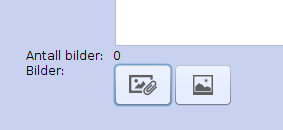
\includegraphics[trim=0cm 0.5cm 0cm 1.6cm,clip]{./img/produktdokumentasjon/bilder/1.png}
 \caption{Utsnitt fra boligbehandlingsvindu. Viser kontroller for opplastning og visning av bilder som er registrert for dette bildeobjektet.}
 \label{fig:bildebahndling}
\end{figure}

\begin{figure}[ht!]
 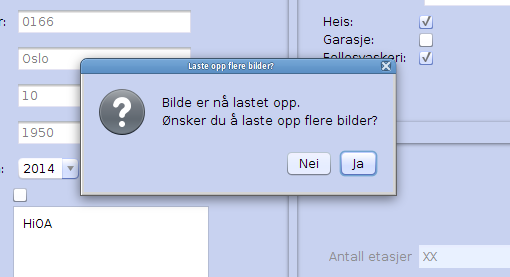
\includegraphics[width=\textwidth,height=\textheight,keepaspectratio,trim= 0cm 2cm 0cm 1cm,clip]{./img/produktdokumentasjon/bilder/2.png}
 \caption{Utsnitt fra boligbehandlingsvindu. Viser forespørsel til bruker (megler) dersom den ønsker å laste opp flere bilder for boligobjetet.}
 \label{fig:lasteoppbilder}
\end{figure}

\begin{figure}[ht!]
 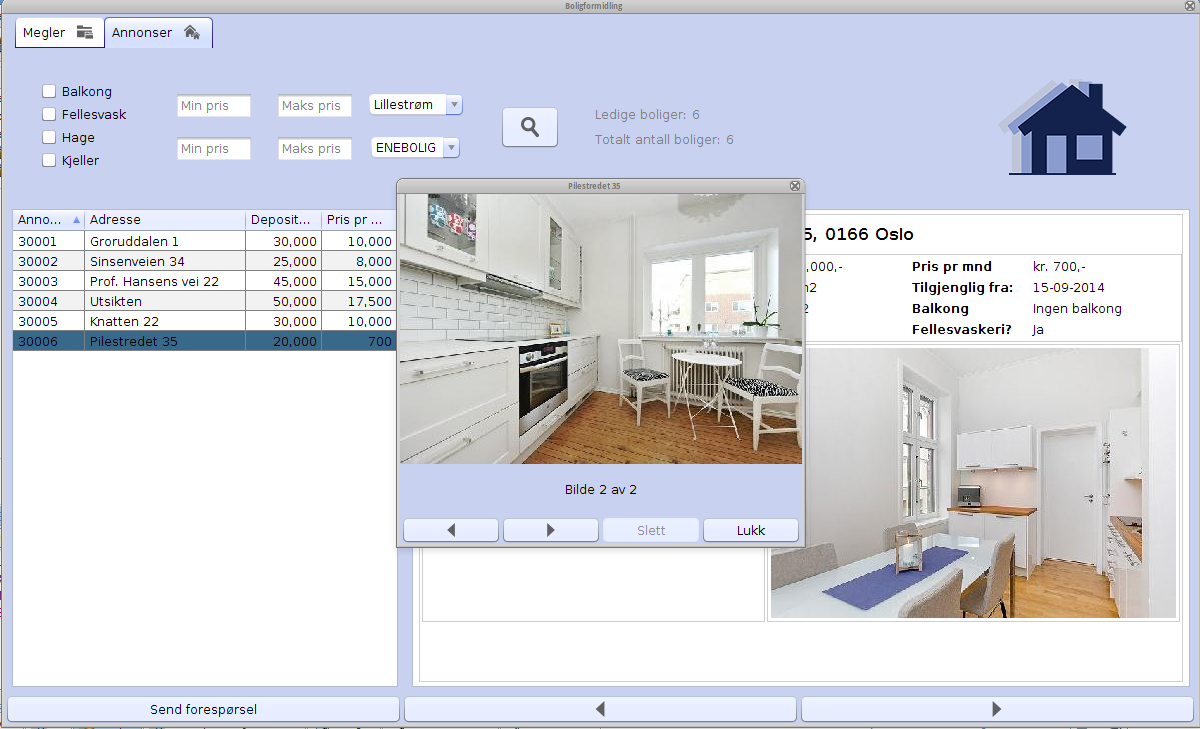
\includegraphics[width=\textwidth,height=\textheight,keepaspectratio]{./img/produktdokumentasjon/bilder/3.png}
 \caption{Bildevisning initialisert gjennom klikk i visningsarea for boligsøker.}
 \label{fig:bildevisning}
\end{figure}

\begin{figure}[ht!]
 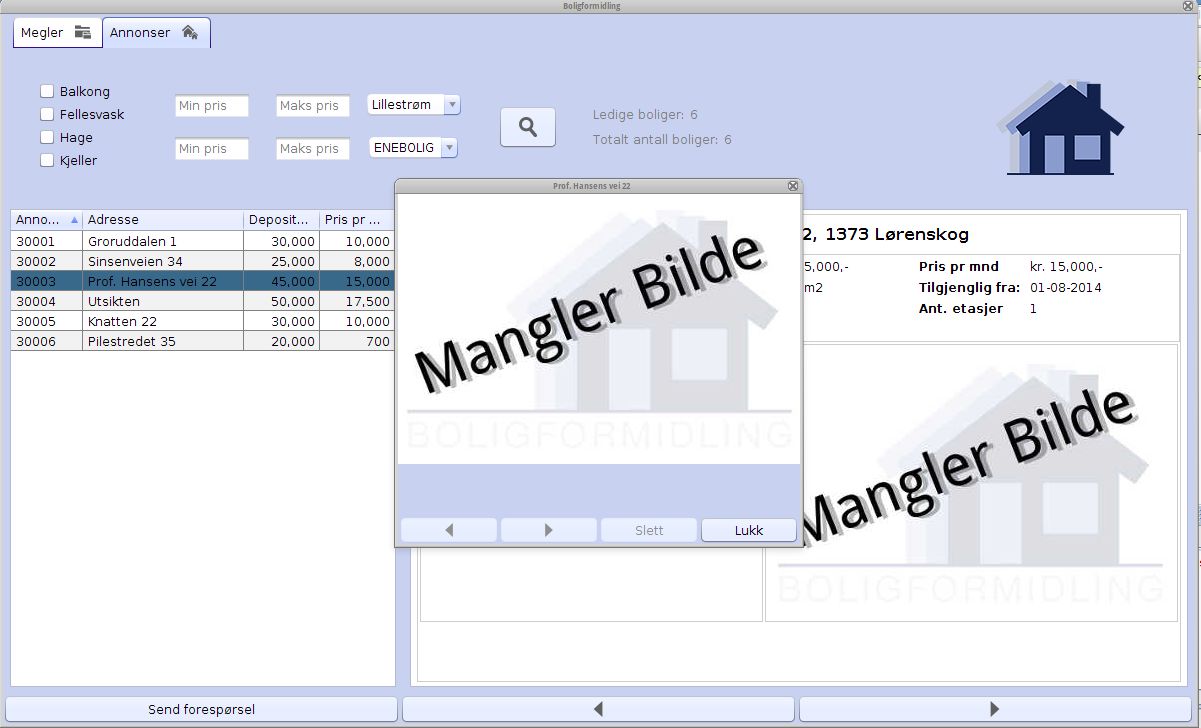
\includegraphics[width=\textwidth,height=\textheight,keepaspectratio]{./img/produktdokumentasjon/bilder/4.png}
 \caption{Eksepel på standardbilde som vises dersom brukeren ikke har lastet opp et bilde etter registrering av en ny bolig.}
 \label{fig:manglerbilde}
\end{figure}

\subsection{Sletting av bilder}
Sletting av bilder er foreløpig ikke implementert. Dersom et boligobjekt blir slettet må gallerimappen til boligen slettes manuellt. Det er tatt høyde for å implementere sletting og mulighet for dette er satt opp i brukergrensesnitet men foreløpig er deaktivert. 